% Options for packages loaded elsewhere
\PassOptionsToPackage{unicode}{hyperref}
\PassOptionsToPackage{hyphens}{url}
%
\documentclass[
]{article}
\usepackage{lmodern}
\usepackage{amssymb,amsmath}
\usepackage{ifxetex,ifluatex}
\ifnum 0\ifxetex 1\fi\ifluatex 1\fi=0 % if pdftex
  \usepackage[T1]{fontenc}
  \usepackage[utf8]{inputenc}
  \usepackage{textcomp} % provide euro and other symbols
\else % if luatex or xetex
  \usepackage{unicode-math}
  \defaultfontfeatures{Scale=MatchLowercase}
  \defaultfontfeatures[\rmfamily]{Ligatures=TeX,Scale=1}
\fi
% Use upquote if available, for straight quotes in verbatim environments
\IfFileExists{upquote.sty}{\usepackage{upquote}}{}
\IfFileExists{microtype.sty}{% use microtype if available
  \usepackage[]{microtype}
  \UseMicrotypeSet[protrusion]{basicmath} % disable protrusion for tt fonts
}{}
\makeatletter
\@ifundefined{KOMAClassName}{% if non-KOMA class
  \IfFileExists{parskip.sty}{%
    \usepackage{parskip}
  }{% else
    \setlength{\parindent}{0pt}
    \setlength{\parskip}{6pt plus 2pt minus 1pt}}
}{% if KOMA class
  \KOMAoptions{parskip=half}}
\makeatother
\usepackage{xcolor}
\IfFileExists{xurl.sty}{\usepackage{xurl}}{} % add URL line breaks if available
\IfFileExists{bookmark.sty}{\usepackage{bookmark}}{\usepackage{hyperref}}
\hypersetup{
  hidelinks,
  pdfcreator={LaTeX via pandoc}}
\urlstyle{same} % disable monospaced font for URLs
\usepackage[margin = 1in]{geometry}
\usepackage{graphicx}
\makeatletter
\def\maxwidth{\ifdim\Gin@nat@width>\linewidth\linewidth\else\Gin@nat@width\fi}
\def\maxheight{\ifdim\Gin@nat@height>\textheight\textheight\else\Gin@nat@height\fi}
\makeatother
% Scale images if necessary, so that they will not overflow the page
% margins by default, and it is still possible to overwrite the defaults
% using explicit options in \includegraphics[width, height, ...]{}
\setkeys{Gin}{width=\maxwidth,height=\maxheight,keepaspectratio}
% Set default figure placement to htbp
\makeatletter
\def\fps@figure{htbp}
\makeatother
\setlength{\emergencystretch}{3em} % prevent overfull lines
\providecommand{\tightlist}{%
  \setlength{\itemsep}{0pt}\setlength{\parskip}{0pt}}
\setcounter{secnumdepth}{-\maxdimen} % remove section numbering

\author{}
\date{\vspace{-2.5em}}

\begin{document}

\hypertarget{methodology}{%
\subsection{3. Methodology}\label{methodology}}

The focus of this thesis is to predict historical prices of bitcoin
using the models listed in Chapter XX. The predictive accuracy of these
obtained predictions are compared using loss functions (Annualized
Sharpe, Diebold Mariano Test, MAE, MSE, RMSE, Mincer-Zarnowitz
Regressions). Then, based on the best models with the most accurate
predictions, trading strategies are worked out to compare with a
buy-and-hold strategy. Finally, we would like to venture into the topic
of explainability and attempt to explain why the chosen models lead to
these outcomes. The procedure of this quantitative study is described in
this chapter.

\begin{itemize}
\tightlist
\item
  Data and Analysis of Bitcoin (BTC/USD)
\item
  Defining the train and test samples (including description about calm
  and volatile phases).
\item
  Calculate predictions with the defined models (AR, NN, RNN, LSTM,
  Emponential Smoothing + NN (Slavek Smyl)).
\item
  Compare Predictions / performance with Realized Data (Annualized
  Sharpe, Diebold Mariano Test, MAE, MSE, RMSE, Mincer-Zarnowitz
  Regressions)
\item
  Explain trading strategies
\item
  Explainability for the best models
\item
  (Backup: Which models work well in which market phases?)
\end{itemize}

\hypertarget{data-and-analysis-of-bitcoin}{%
\subsubsection{3.1. Data and analysis of
Bitcoin}\label{data-and-analysis-of-bitcoin}}

The data in this paper is accessed via yahoofinance provided by
coinmarket \url{https://coinmarketcap.com/}. We use the daily ``closing
price'' of bitcoin in US Dollars with the ticker BTC-USD. Cryptoassets
are tradeble 24 hours a day 256 days a year, there is no real ``closing
price'' for the bitcoin, therefore the ``closing-Price'' is just the
last price of the day evaluated at last timestamp with timeformat UTC.

In chapter \protect\hyperlink{bitcoin}{2.3.} the bitcoin price is
visualized. For processing and analyzing the data in order to fullfill
the weak stationarity assumptions we transform the data into logreturns.

\[\mathrm{LogReturn} = \mathrm{log}(x_{t})-\mathrm{log}(x_{t-1})\]
\includegraphics{04_methodology_files/figure-latex/unnamed-chunk-1-1.pdf}

By computing the autocorrelation oft the log\_returns, there is still
dependence visible in lag 6 and 10. This indicates dependency in
volatility-cluster, to cancel out the effect an ARMA-GARCH model is
fitted to the data and the residuals are standardized by the model
standard-deviation.

\includegraphics{04_methodology_files/figure-latex/unnamed-chunk-2-1.pdf}

\hypertarget{comparison-of-network-architecture}{%
\subsubsection{3.2. Comparison of network
architecture}\label{comparison-of-network-architecture}}

As mentioned in chapter \protect\hyperlink{MLP}{2.1.3.}, choosing an
appropriate network architecture for bitcoin price prediction is a
crucial step in order to achieve useful forecasts while avoiding
overfitting. Due to the complexity as well as the non-linearity of
neural networks, the interpretation cannot be performed intuitively. For
this reason, an approach is pursued in which neural networks with
different numbers of layers and neurons are compared with each other by
using the MSE loss. This allows us to compare accuracy and possibly see
a connection with network architecture. The first plot in figure xy
compares different neural networks with one layer. Networks with a
maximum of six neurons are compared. These different configurations can
be seen on the x-axis. The y-axis shows the MSE values obtained with the
respective optimized model. We use ten different optimizations of each
configuration to get a better idea of a potentially systematic
relationship with the MSE. In the plot, each of the configurations is
drawn using a different color.

\begin{itemize}
\tightlist
\item
  NN for bitcoin prediction
\item
  Non-linear task
\item
  How decide the number of layers and nodes
\item
  Keep in mind rule of thumb
\item
  Test all possible configurations (with realizations = 10) and compare
  the MSE
\end{itemize}

\hypertarget{defining-train-and-test-samples}{%
\subsubsection{3.2. Defining train and test
samples}\label{defining-train-and-test-samples}}

\begin{itemize}
\item
  Describe different phases
\item
  Explain why we set train and test sample like this
\item
  Describe stable and volatile phases and why we should keep that in
  mind for predictions
\end{itemize}

\hypertarget{xy.-benchmark}{%
\paragraph{3.2.xy. Benchmark}\label{xy.-benchmark}}

To compare the models we choose two simple benchmarks the well known buy
and hold and an Ar(1) process as you can see in Figure xy and Figure
xxy.

\hypertarget{xy-evaluating-architecture}{%
\paragraph{3.3.xy Evaluating
architecture}\label{xy-evaluating-architecture}}

In order to find an appropriate model to evaluate our neural net
architecture we needed to compare different architectures of the
network. Therefore we wrote a function which compares all possible
combinations of neurons and layers for a given maximum.

For an easier understanding here is an example:

We want to know all combinations of nets for a maximum of 2 layers with
maximum 2 neurons each. With formula xy we can compute the number of
combinations. In the example case it equals 6 nets, which are plotted in
figure \ref{figure:examples_for_function}, the input layer is cutted
down to two layers for illustration.

\begin{align} \label{eq:complexity}
\net combinations=\sum_{i=1}^{L}N^{i})
\end{align}

with:

\$L = maximum of layers \in \N \$ \$N = maximum of Neurons \in \N \$

\begin{figure}

{\centering 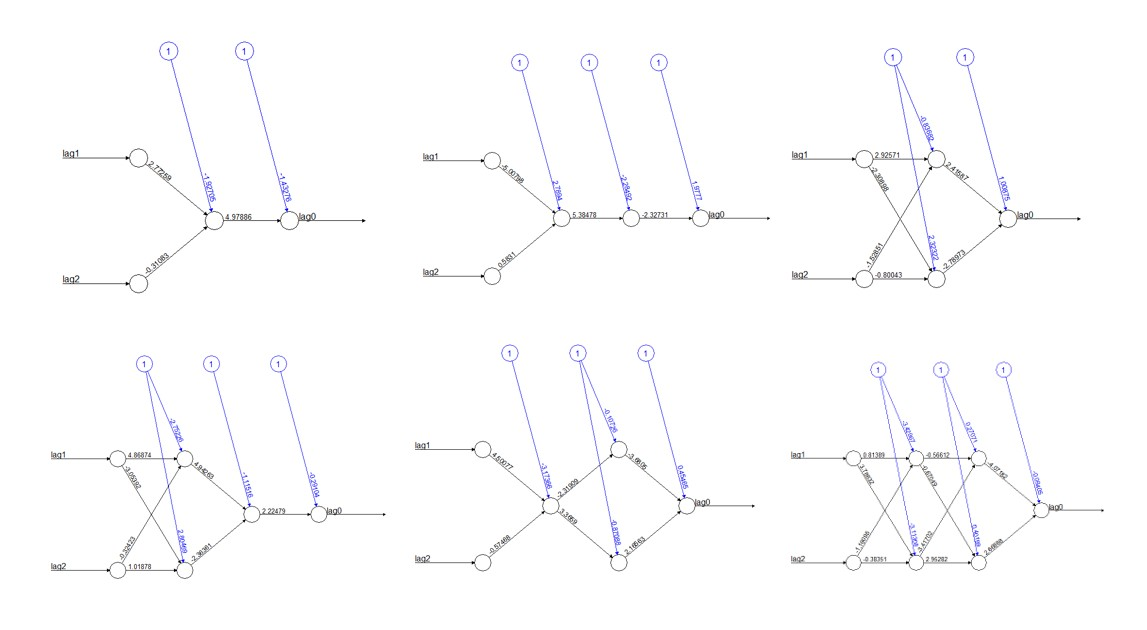
\includegraphics[width=1\linewidth]{images/examples for function} 

}

\caption{Schematic diagram of a perceptron.}\label{fig:examples_for_function}
\end{figure}

The Insample and out of sample MSE are computed and compared. Due to the
"randomness of the networks with specific numbers of layers and neurons,
multiple realisations for every single network are computed to find a
systematic deviation.

Regarding real life application of the model we evaluate performance
over different insample - out of sample

results:

\begin{itemize}
\tightlist
\item
  no need for more complexity, smaller architecture also does the job
\end{itemize}

\hypertarget{trading-strategiesg}{%
\subsubsection{3.4. Trading strategiesg}\label{trading-strategiesg}}

\begin{itemize}
\item
  Define trading strategies
\item
  Sign-trading (daily)
\item
  Vola-gewichtet trading
\item
  Define realistic fee structure for trading (Coinbase Pro, Binance,
  Kraken etc.)
\end{itemize}

\hypertarget{other-cryptocurrency}{%
\subsubsection{3.4.1. Other cryptocurrency}\label{other-cryptocurrency}}

\begin{itemize}
\tightlist
\item
  Test our best model with another time series
\end{itemize}

\hypertarget{explainability}{%
\subsubsection{3.5. Explainability}\label{explainability}}

\begin{itemize}
\item
  Performing the predictions with the two (?) best models
\item
  Include variations to find possible starting points for explainability
  (number of nodes, layers)
\end{itemize}

\hypertarget{relationship-between-accuracy-and-market-phase}{%
\subsubsection{3.6. (Relationship between accuracy and market
phase)}\label{relationship-between-accuracy-and-market-phase}}

\begin{itemize}
\tightlist
\item
  Test
\end{itemize}

\end{document}
